%# -*- coding: utf-8-unix -*-
%%==================================================
%% chapter02.tex for SJTU Master Thesis
%% based on CASthesis
%% modified by wei.jianwen@gmail.com
%% Encoding: UTF-8
%%==================================================
\chapter{设计思路}
\label{chap:example}
基于队列的层级锁(以下简称层级锁)的性能和长期公平性都与线程放置策略有关,而层级锁中现有的两种主要的线程放置策略(紧凑放置和平均放置)分别侧重于锁的性能和长期公平性,在很多场景下两者难以同时兼顾。
本章中我们在对层级锁的锁传递机制及现有线程放置策略做了详细分析,并配合相关的实验验证后,发现现有的线程放置策略的设计初衷对于保证锁的性能或长期公平性是充分而不必要的,在此基础上我们分别针对现有的两种线程放置策略提出了相应的改进思路,并在这两种改进思路的基础上提出了一套在保证锁的性能和长期公平性的前提下额外开销尽可能小的综合线程放置方案。


\section{锁的性能和长期公平性}
在锁集中的高性能应用中,锁很容易成为应用的性能瓶颈,所以锁的性能在很大程度上决定了应用整体的性能\cite{johnson2010decoupling}。锁的性能可以通过其吞吐率来衡量,我们定义锁L的吞吐率为单位时间内L在竞争L的线程间的的平均传递次数,定义单个线程T的吞吐率为单位时间内L在T上的平均传递次数。在锁的竞争激烈的情况下,吞吐率越高表明锁的传递效率越高,锁对应用的性能影响越小。在NUMA架构下,显然影响锁的传递效率的主要因素是访存的非一致性。

锁的长期公平性表示了长远来看锁的传递在线程之间分布的离散程度,在公有云等很多高性能应用场景中锁的长期公平性非常重要。本文中我们用足够长的时间内各个线程拿锁次数的变异系数来衡量锁的长期公平性。变异系数越小表示锁的传递在线程之间的分布越均匀,长期公平性越好。

\section{层级锁的传递机制}
在NUMA架构的机器上,基于队列的锁FIFO的传递顺序造成了频繁的跨NUMA节点的锁传递,而跨NUMA节点的锁传递的巨大开销使得锁的性能受到严重影响。层级锁考虑了NUMA因素,改变了基于队列的锁FIFO的传递顺序,使锁尽可能地在同一个NUMA节点内传递,从而减少锁地跨节点传递进而改善锁的性能。具体来说,层级锁按照以下规则传递:
\begin{itemize}
\item 锁在运行在同一NUMA节点上的线程之间按照FIFO的顺序传递;
\item 锁在NUMA节点之间按照每个节点上当前最早的请求者的FIFO顺序传递;
\item 锁的持有者放锁时将其传给一个本地(同一NUMA节点上)请求者当且仅当以下两个条件同时满足:1)本地节点上当前至少有一个请求者;2)锁在当前节点上的传递次数还未超过预先设定的threshold。否则锁将会被传递到其他节点上。
\end{itemize}
其中设置threshold是为了避免锁在线程之间传递的深度不公平,而为了获取更好的性能,threshold一般被设置为每个NUMA节点上的计算核心数的数倍。

\section{现有线程放置策略}
从以上传递规则可以看出层级锁的性能和长期公平性是与线程在NUMA节点上的分布紧密相关的。现有的线程放置策略中,紧凑放置按照贪心算法将线程依次放置到NUMA节点上,只有当当前节点上没有空余的核时才会将线程放置到一个新的节点上,这样做的好处是使得每个线程放锁时有更大概率在本地节点上找到一个请求者,从而在层级锁的传递机制的基础上进一步避免锁的跨节点传递,获得更好的性能;平均放置将所有线程平均放置在所有节点上,这样做地好处是在层级锁地传递规则下所有线程地地位都是对等的,所以从根本上消除了长期不公平的问题。

\begin{table}[!htbp]
\centering
\bicaption[吞吐率对照]
    {吞吐率}
    {Aggregate Throughput}
  \label{tab:aggregate}
\begin{tabular}{|c|c|c|} 
\hline
\diagbox{暂停时长}{吞吐率(acquisitions/s)}{放置策略}&紧凑放置&平均放置\\
\hline
5000 cycles & 4574093 & 3101512 \\
\hline
500  cycles & 4401877 & 4273903\\
\hline
\end{tabular}
\end{table}
现有的两种线程放置策略分别侧重层级锁的性能和长期公平性,但是在很多场景下难以两者同时兼顾。从层级锁的设计初衷和其的传递规则可以看出,影响层级锁的性能的关键因素是锁的跨NUMA节点传递的频率(比例);而造成锁的长期不公平问题(线程在相关NUMA节点上分布不均匀时)的主要原因是层级锁为了获得高性能而采取得本地偏好的锁传递规则。层级锁为了获得更高性能而采取了本地偏好的传递规则,而本地偏好的传递规则带来了以下两方面的影响:1)为了使本地偏好的传递规则更好地发挥作用(减少锁的跨节点传递比例),线程应该放置地尽可能紧凑;2)线程在NUMA节点上的分布不均匀时会产生长期不公平性问题。

紧凑放置和平均放置分别根据上述两点保证了层级锁地性能和长期公平性,但是很多场景下线程放置很难同时做到紧凑和均匀,所以也就不能同时保证锁的性能和长期公平性。平均放置通过线程在NUMA节点间的均匀放置消除了层级锁的传递规则带来的长期不公平问题,但同时也可能使得层级锁不能充分发挥其本地偏好的特性来减少锁的跨NUMA节点传递,所以也可能会带来性能损失(相比紧凑放置);紧凑放置通过在每个相关节点上放置尽可能多的线程,使得层级锁能够充分利用其本地偏好的锁传递规则来减少锁的跨节点传递,从而保证高性能,但是在线程数不是每个节点上的计算核心数的整数倍数时,层级锁本地偏好地特性可能会造成长期不公平问题。

\begin{table}[!htbp]
  \centering
  \bicaption[变异系数对照]
    {变异系数}
    {Coefficient of Variance}
  \label{tab:CV}
  \begin{tabular}{|c|c|c|} 
  \hline
  \diagbox{暂停时长}{变异系数}{放置策略}&紧凑放置&平均放置\\
   \hline
    5000 cycles & 64.174778\% & 1.939154\%\\
    \hline
    500  cycles & 35.315475\% & 0.036318\%\\
    \hline
  \end{tabular}
\end{table}

\subsection{实验验证}
为了进一步说明现有线程放置策略在层级锁的本地偏好的传递规则下的优势及其局限性,我们做了以下验证性实验。我们的实验跑在Intel Xeon E5上,该机器由四个NUMA节点组成,每个节点上包含八个计算核心。实验的benchmark取自libslock中的stress\_one,实验中用到的锁是C-MCS锁,该锁是一个两层的MCS锁,包括一个全局MCS锁和每个节点上的本地MCS锁。实验中stress\_one被配置为使用12个线程,每个线程重复以下操作:拿锁,写一定大小的缓存,放锁,暂停一段时间。该实验中我们用暂停时间的长短来控制锁的竞争强度的大小,暂停时间越短,线程对锁的请求频率越高,锁的竞争越激烈,实验中用到了两个暂停时间:500时钟周期和5000时钟周期。

表\ref{tab:aggregate}和表\ref{tab:CV}分别展示了紧凑和平均两种线程放置策略在本实验中的两种竞争强度下的吞吐率和变异系数。图\ref{Fig:compact}和图\ref{Fig:even}分别展示了紧凑和平均两种放置策略在本实验中的两种竞争强度下单个线程的吞吐率,其中在平均放置策略中我们只是用了4个NUMA节点中的两个节点。上述两张实验图中每个长条代表单个线程的吞吐率,而不同颜色表示不同的竞争强度。


结合图\ref{Fig:compact}、表\ref{tab:aggregate}和表\ref{tab:CV}可以看出相比平均放置,
紧凑放置在两种暂停时长下都使C-MCS锁获得了更高的吞吐率,但是吞吐率在线程之间地分布严重不均衡,各个线程的拿锁次数的变异系数非常大。结合图\ref{Fig:even}、表\ref{tab:aggregate}和表\ref{tab:CV}可以看出相比紧凑放置,平均放置使得C-MCS锁在两种暂停时长下获得的吞吐率都较小,但是吞吐率在线程之间的分布比较均匀,各个线程拿锁次数的变异系数非常小,说明了线程在节点间的均匀放置可以消除层级锁本地偏好的传递规则带来的长期不公平问题。此外,从图\ref{Fig:compact}中还可以看出同一个NUMA节点上线程的吞吐率之间没有明显的差异,不同NUMA节点上的线程之间吞吐率差别在采用紧凑放置时可以达到十几倍,这种不同节点线程的吞吐率之间的巨大差异正是由层级锁本地偏好的传递规则造成的。

\begin{figure}[htbp]
\centering
\begin{minipage}[t]{0.48\textwidth}
\centering
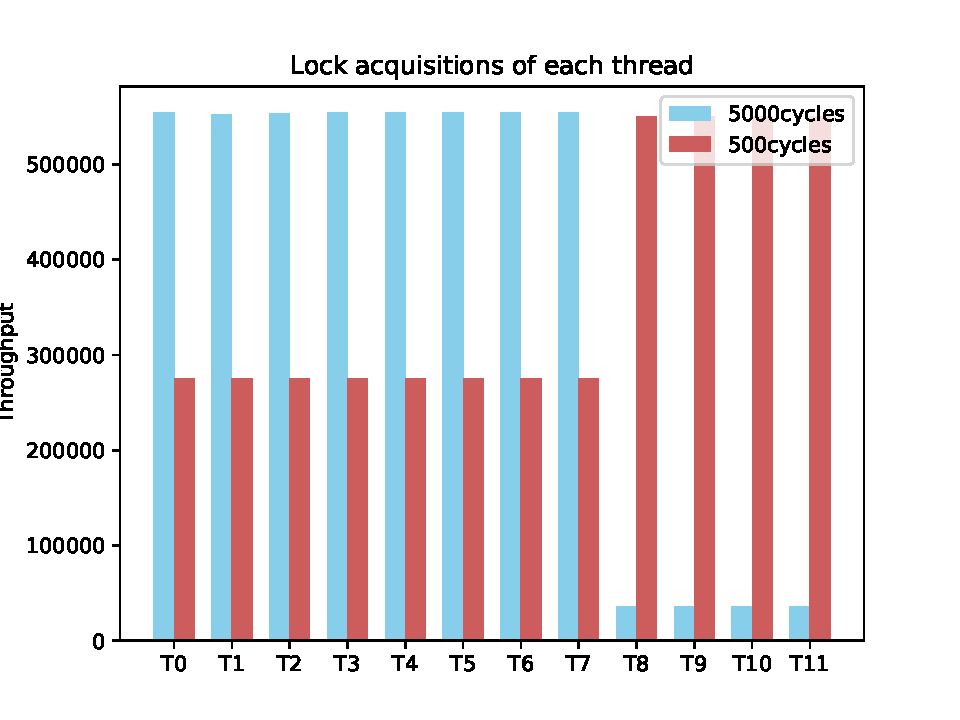
\includegraphics[width=2.8in]{compact.pdf}
\caption{单个线程的吞吐率(紧凑放置)}
	\label{Fig:compact}
\end{minipage}
\begin{minipage}[t]{0.48\textwidth}
\centering
	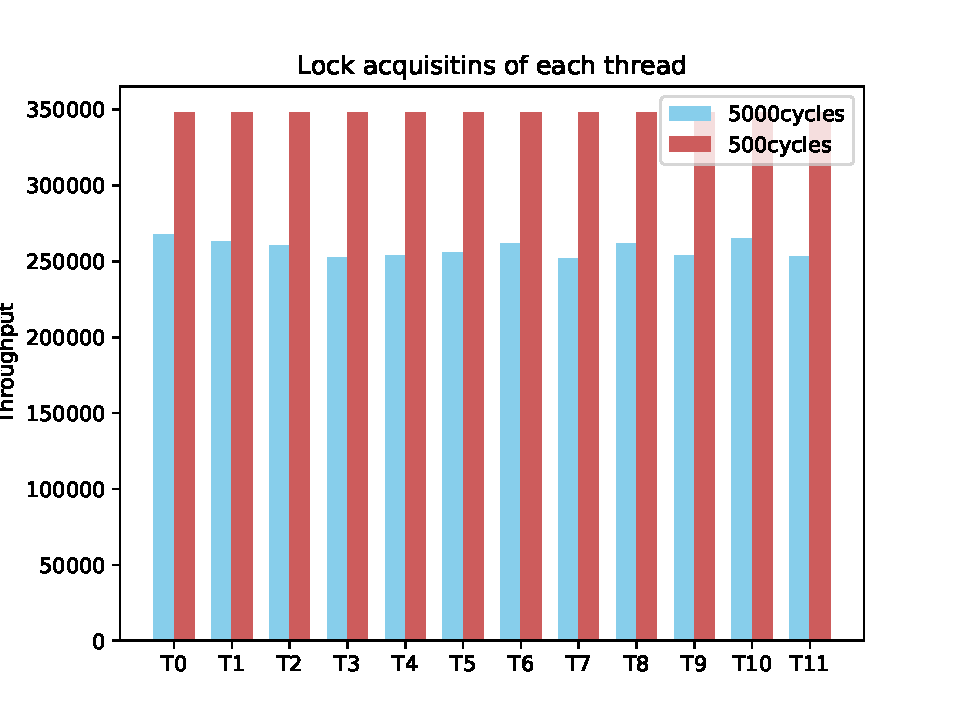
\includegraphics[width=2.8in]{even.pdf}
	\caption{单个线程的吞吐率(平均放置)}
	\label{Fig:even}
\end{minipage}
\end{figure}

\section{动机与改进方案}
从上述对层级锁的传递机制和现有的两种主要的线程放置策略的分析的基础上,本节分别针对现有的两种线程放置策略阐述我们的改进动机和相应的改进方案,在此基础上提出一套综合的改进方案。

\subsection{针对紧凑放置的改进思路}
我们认为,紧凑放置采取的贪心放置算法对于保证锁的高性能是充分而不必要的,具体来说,当每个节点上放置的线程数超过一定数量时,就有可能使得锁一直在该节点上传递直到总的传递次数达到threshold的限制,此时再增加该节点上的线程数量并不能进一步减少锁的跨节点传递,也就不可能进一步改进性能,此时的放置在该节点上的线程数即为Malthusian Locks\cite{dice2017malthusian}中定义的饱和点Sat(saturation point),即能保证某个线程放锁时本地NUMA节点上总有至少一个其余线程在等锁的最小线程数。在此基础上,我们提出了一种介于紧凑放置和平均放置的折衷的放置方案,即将所有线程平均放置到尽可能少的NUMA节点上(而不是所有NUMA节点上),我们称新的放置策略为加强的平均放置(Enhanced Even,简称EE),如果EE放置的结果能使每个节点上放置的线程数达到或超过饱和点Sat,则能同时保证锁的性能和长期公平性。

\subsection{针对平均放置的改进思路}
层级锁的本地偏好的传递机制对于运行在同一节点上的线程是长期公平的(FIFO),而对于运行在不同节点上的线程可能是长期不公平的,也就是锁在线程之间的长期公平与否取决于线程的相对位置,层级锁中现有的两种线程放置策略都是将线程绑定在固定的核上的,所以只有在线程均匀放置到各个节点上(平均放置)时才能保证锁的长期公平性。现有线程放置策略的都是以将线程固定在核上为前提的,假设我们在此基础上加入线程迁移调度,在保持线程分布格局(即每个节点上分布的线程数)不变的情况下,通过定期的交换线程的位置,使得长远来看每个线程在每个节点上运行差不多的时间,那么同样可以保证层级锁的长期公平性。在此基础上,我们设计了一种新的线程放置策略,即有轮换的紧凑放置(Compact With Shift, CWS), CWS在紧凑放置的基础上采用了轮换(shift)机制,即通过定期的交换线程的运行位置来保证长远来看,每个线程在每个节点上运行大致相同的时间,从而同时保证层级锁的性能和长期公平性。

\subsection{综合改进方案}
上述两种改进思路都可以同时保证层级锁的高性能和长期公平性,但是分别存在以下问题:1)EE相比紧凑放置可能会有性能损失,因为EE放置不一定能使得相关NUMA节点上放置的线程数大于等于饱和点Sat;2)CWS相比紧凑放置会引入线程迁移,而线程迁移必将带来额外的开销。所以在此基础上,为了设计出一种能够在各种场景下同时保证层级锁的性能和长期公平性的线程放置方案,我们必须首先解决以下两个问题:
\begin{enumerate}
    \item 如何判断EE放置相比紧凑放置是否有性能损失?即如何获得饱和点Sat的大小。
    \item shift机制的锁造成的线程迁移必须尽可能地小,从而在不对性能产生明显影响的前提下保证长期公平性。
\end{enumerate}
我们将在下一章给出是shift机制的具体流程,而由饱和点的物理意义显然有:
\begin{equation}\label{Eq:sat}
     Sat = (NCS + CS) / CS
\end{equation}
其中CS和NCS分别代表关键区域和非关键区域的长度。在解决了上述两个问题之后,我们就可以在EE放置相比紧凑放置没有性能损失时(即EE放置后每个相关NUMA节点上放置的线程数大于等于Sat)采用EE放置,否则采用CWS放置,从而能够在各种场景下同时保证层级锁的性能和长期公平性。

\section{本章小结}
在这一章中,我们首先说明了锁的性能和长期公平性的衡量标准,接着通过详细的理论分析和实验验证,说明了层级锁本地偏好的传递机制与现有线程放置策略相结合后对锁的性能和长期公平性的影响。在上述分析和验证的基础上说明了现有线程放置策略保证锁的性能或者长期公平性的初衷是充分而不必要的,并且针对性地提出了两种改进方案,然后在此基础上提出了一套在保证锁的性能和长期公平性地前提下额外开销尽可能小的综合线程方案。此即本文提出的竞争感知的混合线程放置框架CAH的雏形,下一章将会对CAH的设计与实现做详细说明。